



\pagenumbering{arabic}
\setcounter{page}{1}

\chapter{Introduction}


\section{Bitcoin}
Bitcoin is the first decentralized virtual currency and by far has adopted the most number of users ~\cite{Nak08}. it is based on cryptographic functions to remove the need of a central bank and regulates the generation of new units. Bitcoin, as a protocol and as a currency, is a really vast subject that most would fall out of the scope of this thesis. In this thesis, I will talk about Bitcoin as the currency and the functionality of the protocol that is needed in order to hold and use Bitcoin as a currency.

This introduction is not an introduction to Bitcoin, but the details of Bitcoin that is needed in this research, Some details has been simplified to prevent going outside the scope of this thesis. Every aspect of Bitcoin that is missing from this introduction has explained through this thesis when the preliminary information of the usage is known to the reader.


\subsection{Bitcoin Address}
Bitcoin address is a random string of 26-35 alphanumeric characters that starts with "1" or "3", that contains digits, uppercase and lowercase letters with the exception of "O", "I" (Uppercase i) , "l" (Lower case L) and the number 0 to prevent visual ambiguity. Bitcoin addresses are commonly shared via QR-Code as it's easier to read with QR-code mobile scanners and it is also implemented in almost all Bitcoin wallets (see figure ~\ref{fig:bitcoinqr}).

\begin{figure}
\centering

\includegraphics[scale=0.8]{fig/bitcoinqr.png}
  \caption{QR-Code representing the bitcoin address "1shaYanre36PBhspFL9zG7nt6tfDhxQ4u"}
\label{fig:bitcoinqr}
\end{figure}

\subsubsection{Public Key}
 In other words, Bitcoin address is 160-bit hash of the public portion of the public and private ECDSA\footnote{Elliptic Curve Digital Signature Algorithm} keypair (see Figure ~\ref{fig:pubkeytoaddr}).

\begin{figure}
\centering
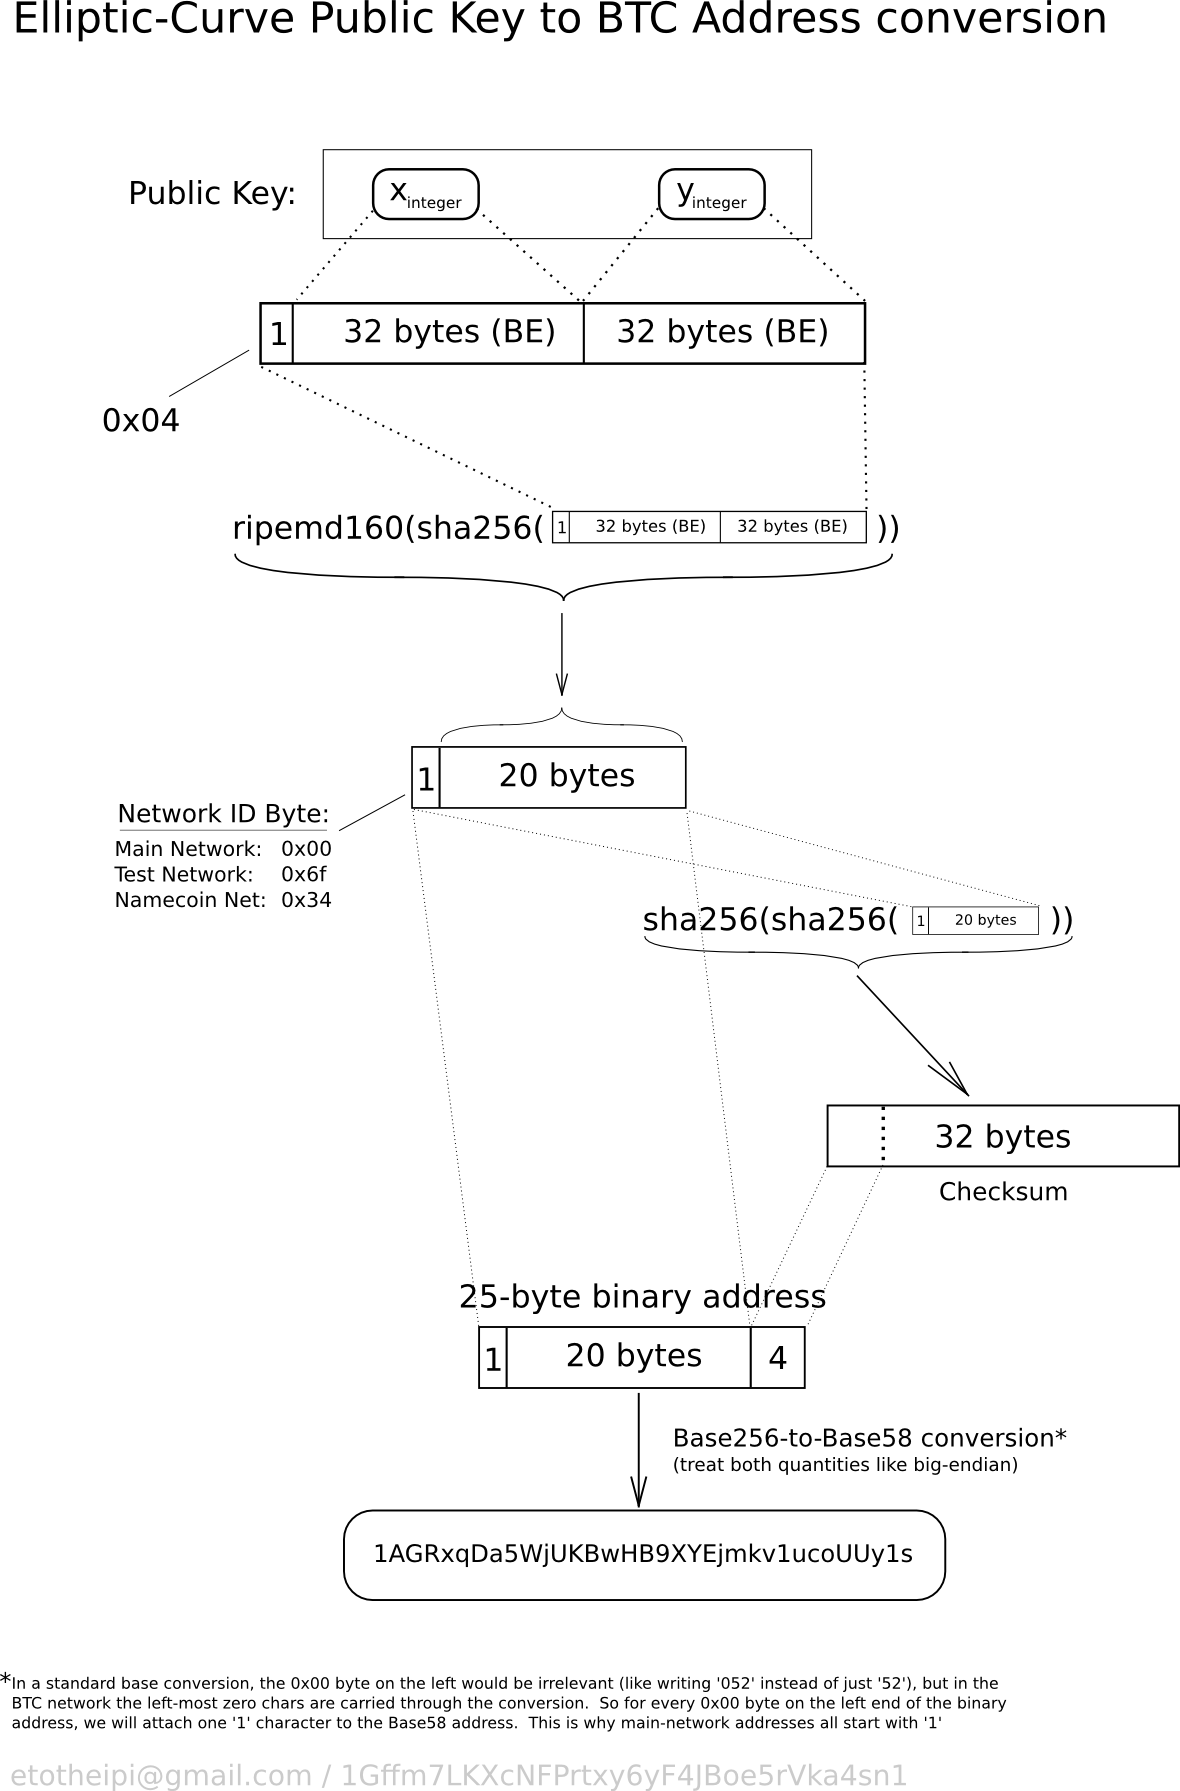
\includegraphics[width=\linewidth]{fig/PubKeyToAddr.png}
  \caption{ECDSA Public key to Bitcoin Address \footnote{\url{https://en.bitcoin.it/wiki/Technical_background_of_version_1_Bitcoin_addresses}}}
\label{fig:pubkeytoaddr}
\end{figure}


\subsubsection{Private Key}
Private key can be any 256 bit number from 0x1 to 0xFFFF FFFF FFFF FFFF FFFF FFFF FFFF FFFE BAAE DCE6 AF48 A03B BFD2 5E8C D036 4140. Basically any number in this range would be valid as the input for secp256k1\footnote{Standards for Efficient Cryptography (SEC) \url{https://en.bitcoin.it/wiki/Secp256k1}} ECDSA standard. This is the secret part of the bitcoin address that should be kept secure and there are already different methods of securing the private key as discussed in Chapter 2. Anyone with the private key has the ability to sign a transaction and spend the bitcoins that are signed with the relevant public key (or bitcoin address). 
Same as Bitcoin addresses and Public keys, Private keys have a shorter format called wallet import format (wif) that is used commonly by most Bitcoin wallets, it contains error checking bits and also have some information about the public key associated to the private key. An example of a private key in wif format would be "5Kb8kLf9zgWQnogidDA76MzPL6TsZZY36hWXMssSzNydYXYB9KF" that would result in "1CC3X2gu58d6wXUWMffpuzN9JAfTUWu4Kj" as the associated bitcoin address.

\fixme{maybe more details on address generation?}


\subsubsection{BIP32}
As Satoshi Nakamoto ~\cite{Nak08} also points out, it's better to generate a new address for each transaction and receive the changes in a new change address( The concept of change addresses would be explained more in chapter 2) to use the pseudonymity of bitcoin. This brought a challenge to Bitcoin wallet client designs as keeping track of all the addresses in the wallet file and also the ability to back up the private keys (More on Chapter 2). 
Bitcoin is an open source project, and to make improvements to the protocol there are Bitcoin Improvement Proposals (BIP) introduced by mostly developers to be implemented in the core code. One important one is BIP32 known as Hierarchical Deterministic Wallets or HD wallets ~\cite{bip32}. It introduce the ability to generate a tree of addresses from a single seed, this could be shown as 0/1 as in branch 0 of the root and branch 1 of the next branch. BIP32 simplifies the backing up process as there is just a seed to be backed up and it's easier to keep track of the addresses, a visualization of how BIP32 is design can be seen in figure ~\ref{fig:bip32}.

\begin{figure}
\centering
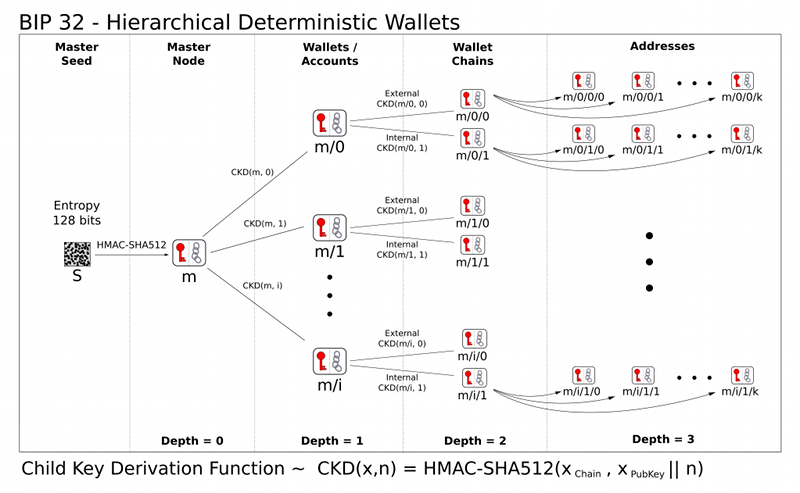
\includegraphics[width=\linewidth]{fig/bip32derivation.png}
  \caption{BIP32 - Hierarchical Deterministic Wallets \footnote{\url{https://github.com/bitcoin/bips/blob/master/bip-0032.mediawiki}}}}
\label{fig:bip32}
\end{figure}


\subsection{Bitcoin Wallet}
This term has been misused in bitcoin sphere as both the file that contains the private keys and also the software client used to do mange bitcoin transactions, this concept has been more discussed in Chapter 2. For the sake of simplicity, we use the term Bitcoin wallet client as in the software used to sign bitcoin transactions with the private key held in Bitcoin wallet file and manage the bitcoin transactions.
The first and official Bitcoin wallet client is Bitcoin QT (Bitcoind as the daemon) that will be explained more on Chapter 2.


\subsection{Confirmation}
When a bitcoin transaction is broadcasted to the network, it should get included in a block by Bitcoin miners. Bitcoin miners are the computers that are using their hashing power to verify each and every transaction within the bitcoin network and include them in a block. Each block would be added to the blockchain with a hash referencing its previous block and everyone in the network should have the consensus that the hash value for the block and the previous one is correct. As soon as the transaction is broadcasted it has 0-confirmation, that means it has not been added to any block, right after it gets included in a block it has 1 confirmation and this increases by each block that gets added to the blockchain.

\begin{figure}
\centering
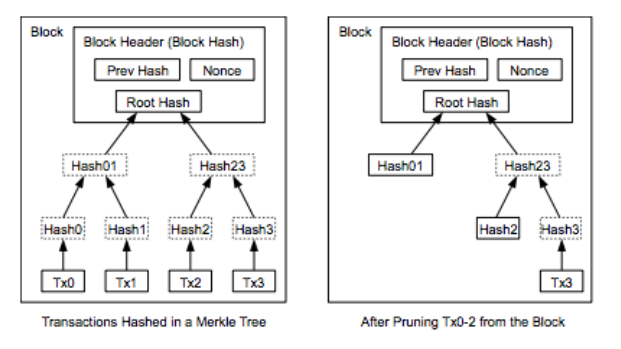
\includegraphics[width=\linewidth]{fig/bitcoinblocks.png}
  \caption{Bitcoin Blocks in the blockchain ~\cite{Nak08}}
\label{fig:bitcoinblocks}
\end{figure}

This is really important to understand that it is possible for a 0-confirmation transaction to stay unconfirmed for a while, depending on how much miner's fee is included in the transaction, miner's tend to chose the transactions with a higher miner's fee to be included in the new block first.

\fixme{double spend attack}

\section{Structure of this thesis}
\fixme{what should go here? talk about why the chapters are the ones that they are??}

\fixme{what else?}


